% Created by tikzDevice version 0.12.3.1 on 2023-04-20 20:50:45
% !TEX encoding = UTF-8 Unicode
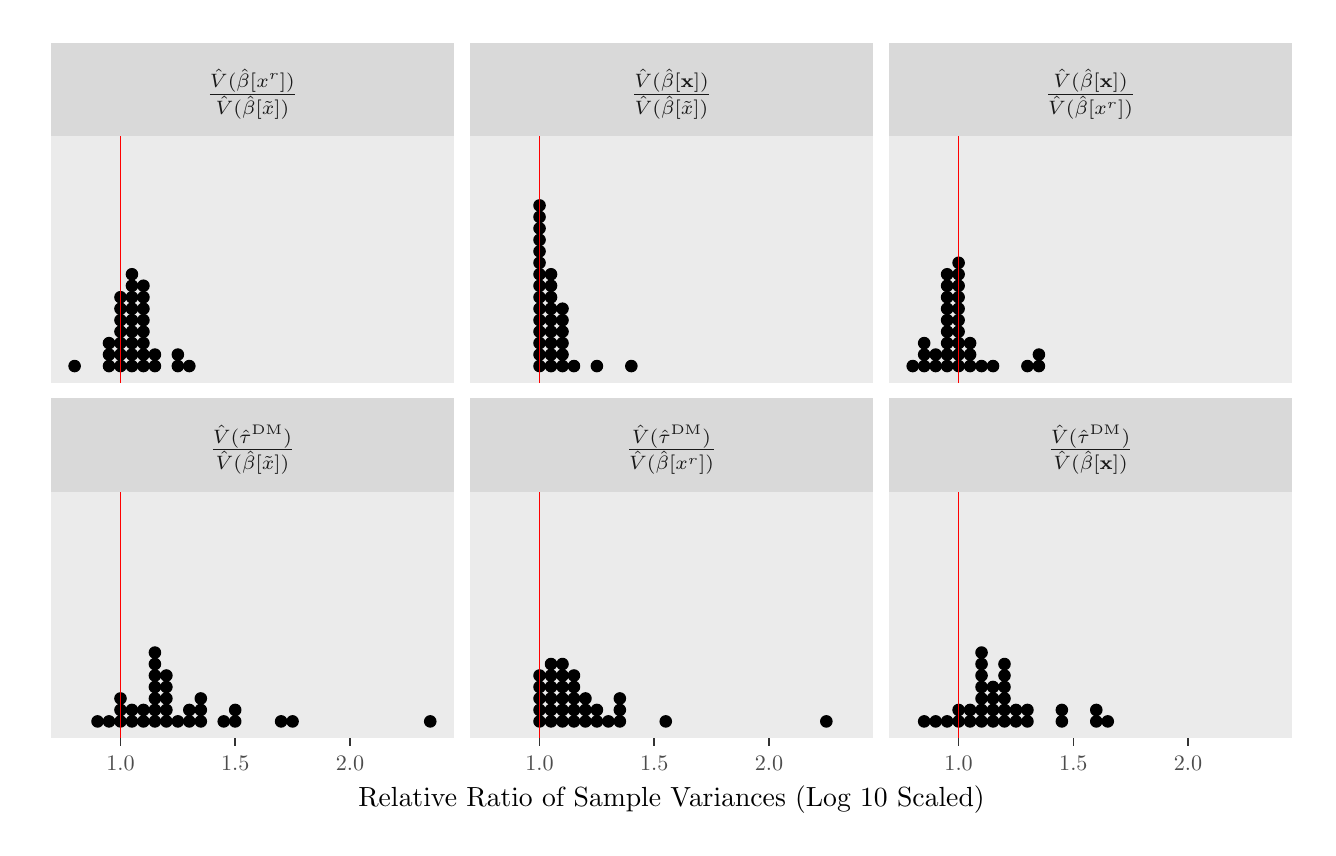
\begin{tikzpicture}[x=1pt,y=1pt]
\definecolor{fillColor}{RGB}{255,255,255}
\path[use as bounding box,fill=fillColor,fill opacity=0.00] (0,0) rectangle (462.53,289.08);
\begin{scope}
\path[clip] (  0.00,  0.00) rectangle (462.53,289.08);
\definecolor{drawColor}{RGB}{255,255,255}
\definecolor{fillColor}{RGB}{255,255,255}

\path[draw=drawColor,line width= 0.6pt,line join=round,line cap=round,fill=fillColor] (  0.00,  0.00) rectangle (462.53,289.08);
\end{scope}
\begin{scope}
\path[clip] (  8.25,160.68) rectangle (154.18,249.78);
\definecolor{fillColor}{gray}{0.92}

\path[fill=fillColor] (  8.25,160.68) rectangle (154.18,249.78);
\definecolor{drawColor}{RGB}{0,0,0}
\definecolor{fillColor}{RGB}{0,0,0}

\path[draw=drawColor,line width= 0.4pt,line join=round,fill=fillColor] ( 16.96,166.80) circle (  2.07);

\path[draw=drawColor,line width= 0.4pt,line join=round,fill=fillColor] ( 29.39,166.80) circle (  2.07);

\path[draw=drawColor,line width= 0.4pt,line join=round,fill=fillColor] ( 29.39,170.95) circle (  2.07);

\path[draw=drawColor,line width= 0.4pt,line join=round,fill=fillColor] ( 29.39,175.09) circle (  2.07);

\path[draw=drawColor,line width= 0.4pt,line join=round,fill=fillColor] ( 33.54,166.80) circle (  2.07);

\path[draw=drawColor,line width= 0.4pt,line join=round,fill=fillColor] ( 33.54,170.95) circle (  2.07);

\path[draw=drawColor,line width= 0.4pt,line join=round,fill=fillColor] ( 33.54,175.09) circle (  2.07);

\path[draw=drawColor,line width= 0.4pt,line join=round,fill=fillColor] ( 33.54,179.24) circle (  2.07);

\path[draw=drawColor,line width= 0.4pt,line join=round,fill=fillColor] ( 33.54,183.38) circle (  2.07);

\path[draw=drawColor,line width= 0.4pt,line join=round,fill=fillColor] ( 33.54,187.53) circle (  2.07);

\path[draw=drawColor,line width= 0.4pt,line join=round,fill=fillColor] ( 33.54,191.67) circle (  2.07);

\path[draw=drawColor,line width= 0.4pt,line join=round,fill=fillColor] ( 37.68,166.80) circle (  2.07);

\path[draw=drawColor,line width= 0.4pt,line join=round,fill=fillColor] ( 37.68,170.95) circle (  2.07);

\path[draw=drawColor,line width= 0.4pt,line join=round,fill=fillColor] ( 37.68,175.09) circle (  2.07);

\path[draw=drawColor,line width= 0.4pt,line join=round,fill=fillColor] ( 37.68,179.24) circle (  2.07);

\path[draw=drawColor,line width= 0.4pt,line join=round,fill=fillColor] ( 37.68,183.38) circle (  2.07);

\path[draw=drawColor,line width= 0.4pt,line join=round,fill=fillColor] ( 37.68,187.53) circle (  2.07);

\path[draw=drawColor,line width= 0.4pt,line join=round,fill=fillColor] ( 37.68,191.67) circle (  2.07);

\path[draw=drawColor,line width= 0.4pt,line join=round,fill=fillColor] ( 37.68,195.82) circle (  2.07);

\path[draw=drawColor,line width= 0.4pt,line join=round,fill=fillColor] ( 37.68,199.97) circle (  2.07);

\path[draw=drawColor,line width= 0.4pt,line join=round,fill=fillColor] ( 41.83,166.80) circle (  2.07);

\path[draw=drawColor,line width= 0.4pt,line join=round,fill=fillColor] ( 41.83,170.95) circle (  2.07);

\path[draw=drawColor,line width= 0.4pt,line join=round,fill=fillColor] ( 41.83,175.09) circle (  2.07);

\path[draw=drawColor,line width= 0.4pt,line join=round,fill=fillColor] ( 41.83,179.24) circle (  2.07);

\path[draw=drawColor,line width= 0.4pt,line join=round,fill=fillColor] ( 41.83,183.38) circle (  2.07);

\path[draw=drawColor,line width= 0.4pt,line join=round,fill=fillColor] ( 41.83,187.53) circle (  2.07);

\path[draw=drawColor,line width= 0.4pt,line join=round,fill=fillColor] ( 41.83,191.67) circle (  2.07);

\path[draw=drawColor,line width= 0.4pt,line join=round,fill=fillColor] ( 41.83,195.82) circle (  2.07);

\path[draw=drawColor,line width= 0.4pt,line join=round,fill=fillColor] ( 45.98,166.80) circle (  2.07);

\path[draw=drawColor,line width= 0.4pt,line join=round,fill=fillColor] ( 45.98,170.95) circle (  2.07);

\path[draw=drawColor,line width= 0.4pt,line join=round,fill=fillColor] ( 54.27,166.80) circle (  2.07);

\path[draw=drawColor,line width= 0.4pt,line join=round,fill=fillColor] ( 54.27,170.95) circle (  2.07);

\path[draw=drawColor,line width= 0.4pt,line join=round,fill=fillColor] ( 58.41,166.80) circle (  2.07);
\definecolor{drawColor}{RGB}{255,0,0}

\path[draw=drawColor,line width= 0.6pt,line join=round] ( 33.54,160.68) -- ( 33.54,249.78);
\end{scope}
\begin{scope}
\path[clip] (  8.25, 32.28) rectangle (154.18,121.38);
\definecolor{fillColor}{gray}{0.92}

\path[fill=fillColor] (  8.25, 32.28) rectangle (154.18,121.38);
\definecolor{drawColor}{RGB}{0,0,0}
\definecolor{fillColor}{RGB}{0,0,0}

\path[draw=drawColor,line width= 0.4pt,line join=round,fill=fillColor] ( 25.25, 38.40) circle (  2.07);

\path[draw=drawColor,line width= 0.4pt,line join=round,fill=fillColor] ( 29.39, 38.40) circle (  2.07);

\path[draw=drawColor,line width= 0.4pt,line join=round,fill=fillColor] ( 33.54, 38.40) circle (  2.07);

\path[draw=drawColor,line width= 0.4pt,line join=round,fill=fillColor] ( 33.54, 42.54) circle (  2.07);

\path[draw=drawColor,line width= 0.4pt,line join=round,fill=fillColor] ( 33.54, 46.69) circle (  2.07);

\path[draw=drawColor,line width= 0.4pt,line join=round,fill=fillColor] ( 37.68, 38.40) circle (  2.07);

\path[draw=drawColor,line width= 0.4pt,line join=round,fill=fillColor] ( 37.68, 42.54) circle (  2.07);

\path[draw=drawColor,line width= 0.4pt,line join=round,fill=fillColor] ( 41.83, 38.40) circle (  2.07);

\path[draw=drawColor,line width= 0.4pt,line join=round,fill=fillColor] ( 41.83, 42.54) circle (  2.07);

\path[draw=drawColor,line width= 0.4pt,line join=round,fill=fillColor] ( 45.98, 38.40) circle (  2.07);

\path[draw=drawColor,line width= 0.4pt,line join=round,fill=fillColor] ( 45.98, 42.54) circle (  2.07);

\path[draw=drawColor,line width= 0.4pt,line join=round,fill=fillColor] ( 45.98, 46.69) circle (  2.07);

\path[draw=drawColor,line width= 0.4pt,line join=round,fill=fillColor] ( 45.98, 50.84) circle (  2.07);

\path[draw=drawColor,line width= 0.4pt,line join=round,fill=fillColor] ( 45.98, 54.98) circle (  2.07);

\path[draw=drawColor,line width= 0.4pt,line join=round,fill=fillColor] ( 45.98, 59.13) circle (  2.07);

\path[draw=drawColor,line width= 0.4pt,line join=round,fill=fillColor] ( 45.98, 63.27) circle (  2.07);

\path[draw=drawColor,line width= 0.4pt,line join=round,fill=fillColor] ( 50.12, 38.40) circle (  2.07);

\path[draw=drawColor,line width= 0.4pt,line join=round,fill=fillColor] ( 50.12, 42.54) circle (  2.07);

\path[draw=drawColor,line width= 0.4pt,line join=round,fill=fillColor] ( 50.12, 46.69) circle (  2.07);

\path[draw=drawColor,line width= 0.4pt,line join=round,fill=fillColor] ( 50.12, 50.84) circle (  2.07);

\path[draw=drawColor,line width= 0.4pt,line join=round,fill=fillColor] ( 50.12, 54.98) circle (  2.07);

\path[draw=drawColor,line width= 0.4pt,line join=round,fill=fillColor] ( 54.27, 38.40) circle (  2.07);

\path[draw=drawColor,line width= 0.4pt,line join=round,fill=fillColor] ( 58.41, 38.40) circle (  2.07);

\path[draw=drawColor,line width= 0.4pt,line join=round,fill=fillColor] ( 58.41, 42.54) circle (  2.07);

\path[draw=drawColor,line width= 0.4pt,line join=round,fill=fillColor] ( 62.56, 38.40) circle (  2.07);

\path[draw=drawColor,line width= 0.4pt,line join=round,fill=fillColor] ( 62.56, 42.54) circle (  2.07);

\path[draw=drawColor,line width= 0.4pt,line join=round,fill=fillColor] ( 62.56, 46.69) circle (  2.07);

\path[draw=drawColor,line width= 0.4pt,line join=round,fill=fillColor] ( 70.85, 38.40) circle (  2.07);

\path[draw=drawColor,line width= 0.4pt,line join=round,fill=fillColor] ( 74.99, 38.40) circle (  2.07);

\path[draw=drawColor,line width= 0.4pt,line join=round,fill=fillColor] ( 74.99, 42.54) circle (  2.07);

\path[draw=drawColor,line width= 0.4pt,line join=round,fill=fillColor] ( 91.58, 38.40) circle (  2.07);

\path[draw=drawColor,line width= 0.4pt,line join=round,fill=fillColor] ( 95.72, 38.40) circle (  2.07);

\path[draw=drawColor,line width= 0.4pt,line join=round,fill=fillColor] (145.47, 38.40) circle (  2.07);
\definecolor{drawColor}{RGB}{255,0,0}

\path[draw=drawColor,line width= 0.6pt,line join=round] ( 33.54, 32.28) -- ( 33.54,121.38);
\end{scope}
\begin{scope}
\path[clip] (159.68,160.68) rectangle (305.60,249.78);
\definecolor{fillColor}{gray}{0.92}

\path[fill=fillColor] (159.68,160.68) rectangle (305.60,249.78);
\definecolor{drawColor}{RGB}{0,0,0}
\definecolor{fillColor}{RGB}{0,0,0}

\path[draw=drawColor,line width= 0.4pt,line join=round,fill=fillColor] (184.96,166.80) circle (  2.07);

\path[draw=drawColor,line width= 0.4pt,line join=round,fill=fillColor] (184.96,170.95) circle (  2.07);

\path[draw=drawColor,line width= 0.4pt,line join=round,fill=fillColor] (184.96,175.09) circle (  2.07);

\path[draw=drawColor,line width= 0.4pt,line join=round,fill=fillColor] (184.96,179.24) circle (  2.07);

\path[draw=drawColor,line width= 0.4pt,line join=round,fill=fillColor] (184.96,183.38) circle (  2.07);

\path[draw=drawColor,line width= 0.4pt,line join=round,fill=fillColor] (184.96,187.53) circle (  2.07);

\path[draw=drawColor,line width= 0.4pt,line join=round,fill=fillColor] (184.96,191.67) circle (  2.07);

\path[draw=drawColor,line width= 0.4pt,line join=round,fill=fillColor] (184.96,195.82) circle (  2.07);

\path[draw=drawColor,line width= 0.4pt,line join=round,fill=fillColor] (184.96,199.97) circle (  2.07);

\path[draw=drawColor,line width= 0.4pt,line join=round,fill=fillColor] (184.96,204.11) circle (  2.07);

\path[draw=drawColor,line width= 0.4pt,line join=round,fill=fillColor] (184.96,208.26) circle (  2.07);

\path[draw=drawColor,line width= 0.4pt,line join=round,fill=fillColor] (184.96,212.40) circle (  2.07);

\path[draw=drawColor,line width= 0.4pt,line join=round,fill=fillColor] (184.96,216.55) circle (  2.07);

\path[draw=drawColor,line width= 0.4pt,line join=round,fill=fillColor] (184.96,220.69) circle (  2.07);

\path[draw=drawColor,line width= 0.4pt,line join=round,fill=fillColor] (184.96,224.84) circle (  2.07);

\path[draw=drawColor,line width= 0.4pt,line join=round,fill=fillColor] (189.11,166.80) circle (  2.07);

\path[draw=drawColor,line width= 0.4pt,line join=round,fill=fillColor] (189.11,170.95) circle (  2.07);

\path[draw=drawColor,line width= 0.4pt,line join=round,fill=fillColor] (189.11,175.09) circle (  2.07);

\path[draw=drawColor,line width= 0.4pt,line join=round,fill=fillColor] (189.11,179.24) circle (  2.07);

\path[draw=drawColor,line width= 0.4pt,line join=round,fill=fillColor] (189.11,183.38) circle (  2.07);

\path[draw=drawColor,line width= 0.4pt,line join=round,fill=fillColor] (189.11,187.53) circle (  2.07);

\path[draw=drawColor,line width= 0.4pt,line join=round,fill=fillColor] (189.11,191.67) circle (  2.07);

\path[draw=drawColor,line width= 0.4pt,line join=round,fill=fillColor] (189.11,195.82) circle (  2.07);

\path[draw=drawColor,line width= 0.4pt,line join=round,fill=fillColor] (189.11,199.97) circle (  2.07);

\path[draw=drawColor,line width= 0.4pt,line join=round,fill=fillColor] (193.26,166.80) circle (  2.07);

\path[draw=drawColor,line width= 0.4pt,line join=round,fill=fillColor] (193.26,170.95) circle (  2.07);

\path[draw=drawColor,line width= 0.4pt,line join=round,fill=fillColor] (193.26,175.09) circle (  2.07);

\path[draw=drawColor,line width= 0.4pt,line join=round,fill=fillColor] (193.26,179.24) circle (  2.07);

\path[draw=drawColor,line width= 0.4pt,line join=round,fill=fillColor] (193.26,183.38) circle (  2.07);

\path[draw=drawColor,line width= 0.4pt,line join=round,fill=fillColor] (193.26,187.53) circle (  2.07);

\path[draw=drawColor,line width= 0.4pt,line join=round,fill=fillColor] (197.40,166.80) circle (  2.07);

\path[draw=drawColor,line width= 0.4pt,line join=round,fill=fillColor] (205.69,166.80) circle (  2.07);

\path[draw=drawColor,line width= 0.4pt,line join=round,fill=fillColor] (218.13,166.80) circle (  2.07);
\definecolor{drawColor}{RGB}{255,0,0}

\path[draw=drawColor,line width= 0.6pt,line join=round] (184.96,160.68) -- (184.96,249.78);
\end{scope}
\begin{scope}
\path[clip] (159.68, 32.28) rectangle (305.60,121.38);
\definecolor{fillColor}{gray}{0.92}

\path[fill=fillColor] (159.68, 32.28) rectangle (305.60,121.38);
\definecolor{drawColor}{RGB}{0,0,0}
\definecolor{fillColor}{RGB}{0,0,0}

\path[draw=drawColor,line width= 0.4pt,line join=round,fill=fillColor] (184.96, 38.40) circle (  2.07);

\path[draw=drawColor,line width= 0.4pt,line join=round,fill=fillColor] (184.96, 42.54) circle (  2.07);

\path[draw=drawColor,line width= 0.4pt,line join=round,fill=fillColor] (184.96, 46.69) circle (  2.07);

\path[draw=drawColor,line width= 0.4pt,line join=round,fill=fillColor] (184.96, 50.84) circle (  2.07);

\path[draw=drawColor,line width= 0.4pt,line join=round,fill=fillColor] (184.96, 54.98) circle (  2.07);

\path[draw=drawColor,line width= 0.4pt,line join=round,fill=fillColor] (189.11, 38.40) circle (  2.07);

\path[draw=drawColor,line width= 0.4pt,line join=round,fill=fillColor] (189.11, 42.54) circle (  2.07);

\path[draw=drawColor,line width= 0.4pt,line join=round,fill=fillColor] (189.11, 46.69) circle (  2.07);

\path[draw=drawColor,line width= 0.4pt,line join=round,fill=fillColor] (189.11, 50.84) circle (  2.07);

\path[draw=drawColor,line width= 0.4pt,line join=round,fill=fillColor] (189.11, 54.98) circle (  2.07);

\path[draw=drawColor,line width= 0.4pt,line join=round,fill=fillColor] (189.11, 59.13) circle (  2.07);

\path[draw=drawColor,line width= 0.4pt,line join=round,fill=fillColor] (193.26, 38.40) circle (  2.07);

\path[draw=drawColor,line width= 0.4pt,line join=round,fill=fillColor] (193.26, 42.54) circle (  2.07);

\path[draw=drawColor,line width= 0.4pt,line join=round,fill=fillColor] (193.26, 46.69) circle (  2.07);

\path[draw=drawColor,line width= 0.4pt,line join=round,fill=fillColor] (193.26, 50.84) circle (  2.07);

\path[draw=drawColor,line width= 0.4pt,line join=round,fill=fillColor] (193.26, 54.98) circle (  2.07);

\path[draw=drawColor,line width= 0.4pt,line join=round,fill=fillColor] (193.26, 59.13) circle (  2.07);

\path[draw=drawColor,line width= 0.4pt,line join=round,fill=fillColor] (197.40, 38.40) circle (  2.07);

\path[draw=drawColor,line width= 0.4pt,line join=round,fill=fillColor] (197.40, 42.54) circle (  2.07);

\path[draw=drawColor,line width= 0.4pt,line join=round,fill=fillColor] (197.40, 46.69) circle (  2.07);

\path[draw=drawColor,line width= 0.4pt,line join=round,fill=fillColor] (197.40, 50.84) circle (  2.07);

\path[draw=drawColor,line width= 0.4pt,line join=round,fill=fillColor] (197.40, 54.98) circle (  2.07);

\path[draw=drawColor,line width= 0.4pt,line join=round,fill=fillColor] (201.55, 38.40) circle (  2.07);

\path[draw=drawColor,line width= 0.4pt,line join=round,fill=fillColor] (201.55, 42.54) circle (  2.07);

\path[draw=drawColor,line width= 0.4pt,line join=round,fill=fillColor] (201.55, 46.69) circle (  2.07);

\path[draw=drawColor,line width= 0.4pt,line join=round,fill=fillColor] (205.69, 38.40) circle (  2.07);

\path[draw=drawColor,line width= 0.4pt,line join=round,fill=fillColor] (205.69, 42.54) circle (  2.07);

\path[draw=drawColor,line width= 0.4pt,line join=round,fill=fillColor] (209.84, 38.40) circle (  2.07);

\path[draw=drawColor,line width= 0.4pt,line join=round,fill=fillColor] (213.98, 38.40) circle (  2.07);

\path[draw=drawColor,line width= 0.4pt,line join=round,fill=fillColor] (213.98, 42.54) circle (  2.07);

\path[draw=drawColor,line width= 0.4pt,line join=round,fill=fillColor] (213.98, 46.69) circle (  2.07);

\path[draw=drawColor,line width= 0.4pt,line join=round,fill=fillColor] (230.57, 38.40) circle (  2.07);

\path[draw=drawColor,line width= 0.4pt,line join=round,fill=fillColor] (288.60, 38.40) circle (  2.07);
\definecolor{drawColor}{RGB}{255,0,0}

\path[draw=drawColor,line width= 0.6pt,line join=round] (184.96, 32.28) -- (184.96,121.38);
\end{scope}
\begin{scope}
\path[clip] (311.10,160.68) rectangle (457.03,249.78);
\definecolor{fillColor}{gray}{0.92}

\path[fill=fillColor] (311.10,160.68) rectangle (457.03,249.78);
\definecolor{drawColor}{RGB}{0,0,0}
\definecolor{fillColor}{RGB}{0,0,0}

\path[draw=drawColor,line width= 0.4pt,line join=round,fill=fillColor] (319.81,166.80) circle (  2.07);

\path[draw=drawColor,line width= 0.4pt,line join=round,fill=fillColor] (323.95,166.80) circle (  2.07);

\path[draw=drawColor,line width= 0.4pt,line join=round,fill=fillColor] (323.95,170.95) circle (  2.07);

\path[draw=drawColor,line width= 0.4pt,line join=round,fill=fillColor] (323.95,175.09) circle (  2.07);

\path[draw=drawColor,line width= 0.4pt,line join=round,fill=fillColor] (328.10,166.80) circle (  2.07);

\path[draw=drawColor,line width= 0.4pt,line join=round,fill=fillColor] (328.10,170.95) circle (  2.07);

\path[draw=drawColor,line width= 0.4pt,line join=round,fill=fillColor] (332.24,166.80) circle (  2.07);

\path[draw=drawColor,line width= 0.4pt,line join=round,fill=fillColor] (332.24,170.95) circle (  2.07);

\path[draw=drawColor,line width= 0.4pt,line join=round,fill=fillColor] (332.24,175.09) circle (  2.07);

\path[draw=drawColor,line width= 0.4pt,line join=round,fill=fillColor] (332.24,179.24) circle (  2.07);

\path[draw=drawColor,line width= 0.4pt,line join=round,fill=fillColor] (332.24,183.38) circle (  2.07);

\path[draw=drawColor,line width= 0.4pt,line join=round,fill=fillColor] (332.24,187.53) circle (  2.07);

\path[draw=drawColor,line width= 0.4pt,line join=round,fill=fillColor] (332.24,191.67) circle (  2.07);

\path[draw=drawColor,line width= 0.4pt,line join=round,fill=fillColor] (332.24,195.82) circle (  2.07);

\path[draw=drawColor,line width= 0.4pt,line join=round,fill=fillColor] (332.24,199.97) circle (  2.07);

\path[draw=drawColor,line width= 0.4pt,line join=round,fill=fillColor] (336.39,166.80) circle (  2.07);

\path[draw=drawColor,line width= 0.4pt,line join=round,fill=fillColor] (336.39,170.95) circle (  2.07);

\path[draw=drawColor,line width= 0.4pt,line join=round,fill=fillColor] (336.39,175.09) circle (  2.07);

\path[draw=drawColor,line width= 0.4pt,line join=round,fill=fillColor] (336.39,179.24) circle (  2.07);

\path[draw=drawColor,line width= 0.4pt,line join=round,fill=fillColor] (336.39,183.38) circle (  2.07);

\path[draw=drawColor,line width= 0.4pt,line join=round,fill=fillColor] (336.39,187.53) circle (  2.07);

\path[draw=drawColor,line width= 0.4pt,line join=round,fill=fillColor] (336.39,191.67) circle (  2.07);

\path[draw=drawColor,line width= 0.4pt,line join=round,fill=fillColor] (336.39,195.82) circle (  2.07);

\path[draw=drawColor,line width= 0.4pt,line join=round,fill=fillColor] (336.39,199.97) circle (  2.07);

\path[draw=drawColor,line width= 0.4pt,line join=round,fill=fillColor] (336.39,204.11) circle (  2.07);

\path[draw=drawColor,line width= 0.4pt,line join=round,fill=fillColor] (340.54,166.80) circle (  2.07);

\path[draw=drawColor,line width= 0.4pt,line join=round,fill=fillColor] (340.54,170.95) circle (  2.07);

\path[draw=drawColor,line width= 0.4pt,line join=round,fill=fillColor] (340.54,175.09) circle (  2.07);

\path[draw=drawColor,line width= 0.4pt,line join=round,fill=fillColor] (344.68,166.80) circle (  2.07);

\path[draw=drawColor,line width= 0.4pt,line join=round,fill=fillColor] (348.83,166.80) circle (  2.07);

\path[draw=drawColor,line width= 0.4pt,line join=round,fill=fillColor] (361.26,166.80) circle (  2.07);

\path[draw=drawColor,line width= 0.4pt,line join=round,fill=fillColor] (365.41,166.80) circle (  2.07);

\path[draw=drawColor,line width= 0.4pt,line join=round,fill=fillColor] (365.41,170.95) circle (  2.07);
\definecolor{drawColor}{RGB}{255,0,0}

\path[draw=drawColor,line width= 0.6pt,line join=round] (336.39,160.68) -- (336.39,249.78);
\end{scope}
\begin{scope}
\path[clip] (311.10, 32.28) rectangle (457.03,121.38);
\definecolor{fillColor}{gray}{0.92}

\path[fill=fillColor] (311.10, 32.28) rectangle (457.03,121.38);
\definecolor{drawColor}{RGB}{0,0,0}
\definecolor{fillColor}{RGB}{0,0,0}

\path[draw=drawColor,line width= 0.4pt,line join=round,fill=fillColor] (323.95, 38.40) circle (  2.07);

\path[draw=drawColor,line width= 0.4pt,line join=round,fill=fillColor] (328.10, 38.40) circle (  2.07);

\path[draw=drawColor,line width= 0.4pt,line join=round,fill=fillColor] (332.24, 38.40) circle (  2.07);

\path[draw=drawColor,line width= 0.4pt,line join=round,fill=fillColor] (336.39, 38.40) circle (  2.07);

\path[draw=drawColor,line width= 0.4pt,line join=round,fill=fillColor] (336.39, 42.54) circle (  2.07);

\path[draw=drawColor,line width= 0.4pt,line join=round,fill=fillColor] (340.54, 38.40) circle (  2.07);

\path[draw=drawColor,line width= 0.4pt,line join=round,fill=fillColor] (340.54, 42.54) circle (  2.07);

\path[draw=drawColor,line width= 0.4pt,line join=round,fill=fillColor] (344.68, 38.40) circle (  2.07);

\path[draw=drawColor,line width= 0.4pt,line join=round,fill=fillColor] (344.68, 42.54) circle (  2.07);

\path[draw=drawColor,line width= 0.4pt,line join=round,fill=fillColor] (344.68, 46.69) circle (  2.07);

\path[draw=drawColor,line width= 0.4pt,line join=round,fill=fillColor] (344.68, 50.84) circle (  2.07);

\path[draw=drawColor,line width= 0.4pt,line join=round,fill=fillColor] (344.68, 54.98) circle (  2.07);

\path[draw=drawColor,line width= 0.4pt,line join=round,fill=fillColor] (344.68, 59.13) circle (  2.07);

\path[draw=drawColor,line width= 0.4pt,line join=round,fill=fillColor] (344.68, 63.27) circle (  2.07);

\path[draw=drawColor,line width= 0.4pt,line join=round,fill=fillColor] (348.83, 38.40) circle (  2.07);

\path[draw=drawColor,line width= 0.4pt,line join=round,fill=fillColor] (348.83, 42.54) circle (  2.07);

\path[draw=drawColor,line width= 0.4pt,line join=round,fill=fillColor] (348.83, 46.69) circle (  2.07);

\path[draw=drawColor,line width= 0.4pt,line join=round,fill=fillColor] (348.83, 50.84) circle (  2.07);

\path[draw=drawColor,line width= 0.4pt,line join=round,fill=fillColor] (352.97, 38.40) circle (  2.07);

\path[draw=drawColor,line width= 0.4pt,line join=round,fill=fillColor] (352.97, 42.54) circle (  2.07);

\path[draw=drawColor,line width= 0.4pt,line join=round,fill=fillColor] (352.97, 46.69) circle (  2.07);

\path[draw=drawColor,line width= 0.4pt,line join=round,fill=fillColor] (352.97, 50.84) circle (  2.07);

\path[draw=drawColor,line width= 0.4pt,line join=round,fill=fillColor] (352.97, 54.98) circle (  2.07);

\path[draw=drawColor,line width= 0.4pt,line join=round,fill=fillColor] (352.97, 59.13) circle (  2.07);

\path[draw=drawColor,line width= 0.4pt,line join=round,fill=fillColor] (357.12, 38.40) circle (  2.07);

\path[draw=drawColor,line width= 0.4pt,line join=round,fill=fillColor] (357.12, 42.54) circle (  2.07);

\path[draw=drawColor,line width= 0.4pt,line join=round,fill=fillColor] (361.26, 38.40) circle (  2.07);

\path[draw=drawColor,line width= 0.4pt,line join=round,fill=fillColor] (361.26, 42.54) circle (  2.07);

\path[draw=drawColor,line width= 0.4pt,line join=round,fill=fillColor] (373.70, 38.40) circle (  2.07);

\path[draw=drawColor,line width= 0.4pt,line join=round,fill=fillColor] (373.70, 42.54) circle (  2.07);

\path[draw=drawColor,line width= 0.4pt,line join=round,fill=fillColor] (386.14, 38.40) circle (  2.07);

\path[draw=drawColor,line width= 0.4pt,line join=round,fill=fillColor] (386.14, 42.54) circle (  2.07);

\path[draw=drawColor,line width= 0.4pt,line join=round,fill=fillColor] (390.28, 38.40) circle (  2.07);
\definecolor{drawColor}{RGB}{255,0,0}

\path[draw=drawColor,line width= 0.6pt,line join=round] (336.39, 32.28) -- (336.39,121.38);
\end{scope}
\begin{scope}
\path[clip] (  8.25,121.38) rectangle (154.18,155.18);
\definecolor{fillColor}{gray}{0.85}

\path[fill=fillColor] (  8.25,121.38) rectangle (154.18,155.18);
\definecolor{drawColor}{gray}{0.10}

\node[text=drawColor,anchor=base,inner sep=0pt, outer sep=0pt, scale=  1.00] at ( 81.21,141.35) {};

\node[text=drawColor,anchor=base,inner sep=0pt, outer sep=0pt, scale=  1.00] at ( 81.21,134.15) {$\frac{\hat{\mathbb{V}}(\hat{\tau}^{\mathrm{DM}})}{\hat{\mathbb{V}}(\hat{\beta}[\tilde{x}])}$};

\node[text=drawColor,anchor=base,inner sep=0pt, outer sep=0pt, scale=  1.00] at ( 81.21,126.95) {};
\end{scope}
\begin{scope}
\path[clip] (159.68,121.38) rectangle (305.60,155.18);
\definecolor{fillColor}{gray}{0.85}

\path[fill=fillColor] (159.68,121.38) rectangle (305.60,155.18);
\definecolor{drawColor}{gray}{0.10}

\node[text=drawColor,anchor=base,inner sep=0pt, outer sep=0pt, scale=  1.00] at (232.64,141.35) {};

\node[text=drawColor,anchor=base,inner sep=0pt, outer sep=0pt, scale=  1.00] at (232.64,134.15) {$\frac{\hat{\mathbb{V}}(\hat{\tau}^{\mathrm{DM}})}{\hat{\mathbb{V}}(\hat{\beta}[x^r])}$};

\node[text=drawColor,anchor=base,inner sep=0pt, outer sep=0pt, scale=  1.00] at (232.64,126.95) {};
\end{scope}
\begin{scope}
\path[clip] (311.10,121.38) rectangle (457.03,155.18);
\definecolor{fillColor}{gray}{0.85}

\path[fill=fillColor] (311.10,121.38) rectangle (457.03,155.18);
\definecolor{drawColor}{gray}{0.10}

\node[text=drawColor,anchor=base,inner sep=0pt, outer sep=0pt, scale=  1.00] at (384.06,141.35) {};

\node[text=drawColor,anchor=base,inner sep=0pt, outer sep=0pt, scale=  1.00] at (384.06,134.15) {$\frac{\hat{\mathbb{V}}(\hat{\tau}^{\mathrm{DM}})}{\hat{\mathbb{V}}(\hat{\beta}[\mathbf{x}])}$};

\node[text=drawColor,anchor=base,inner sep=0pt, outer sep=0pt, scale=  1.00] at (384.06,126.95) {};
\end{scope}
\begin{scope}
\path[clip] (  8.25,249.78) rectangle (154.18,283.58);
\definecolor{fillColor}{gray}{0.85}

\path[fill=fillColor] (  8.25,249.78) rectangle (154.18,283.58);
\definecolor{drawColor}{gray}{0.10}

\node[text=drawColor,anchor=base,inner sep=0pt, outer sep=0pt, scale=  1.00] at ( 81.21,269.75) {};

\node[text=drawColor,anchor=base,inner sep=0pt, outer sep=0pt, scale=  1.00] at ( 81.21,262.55) {$\frac{\hat{\mathbb{V}}(\hat{\beta}[x^r])}{\hat{\mathbb{V}}(\hat{\beta}[\tilde{x}])}$};

\node[text=drawColor,anchor=base,inner sep=0pt, outer sep=0pt, scale=  1.00] at ( 81.21,255.35) {};
\end{scope}
\begin{scope}
\path[clip] (159.68,249.78) rectangle (305.60,283.58);
\definecolor{fillColor}{gray}{0.85}

\path[fill=fillColor] (159.68,249.78) rectangle (305.60,283.58);
\definecolor{drawColor}{gray}{0.10}

\node[text=drawColor,anchor=base,inner sep=0pt, outer sep=0pt, scale=  1.00] at (232.64,269.75) {};

\node[text=drawColor,anchor=base,inner sep=0pt, outer sep=0pt, scale=  1.00] at (232.64,262.55) {$\frac{\hat{\mathbb{V}}(\hat{\beta}[\mathbf{x}])}{\hat{\mathbb{V}}(\hat{\beta}[\tilde{x}])}$};

\node[text=drawColor,anchor=base,inner sep=0pt, outer sep=0pt, scale=  1.00] at (232.64,255.35) {};
\end{scope}
\begin{scope}
\path[clip] (311.10,249.78) rectangle (457.03,283.58);
\definecolor{fillColor}{gray}{0.85}

\path[fill=fillColor] (311.10,249.78) rectangle (457.03,283.58);
\definecolor{drawColor}{gray}{0.10}

\node[text=drawColor,anchor=base,inner sep=0pt, outer sep=0pt, scale=  1.00] at (384.06,269.75) {};

\node[text=drawColor,anchor=base,inner sep=0pt, outer sep=0pt, scale=  1.00] at (384.06,262.55) {$\frac{\hat{\mathbb{V}}(\hat{\beta}[\mathbf{x}])}{\hat{\mathbb{V}}(\hat{\beta}[x^r])}$};

\node[text=drawColor,anchor=base,inner sep=0pt, outer sep=0pt, scale=  1.00] at (384.06,255.35) {};
\end{scope}
\begin{scope}
\path[clip] (  0.00,  0.00) rectangle (462.53,289.08);
\definecolor{drawColor}{gray}{0.20}

\path[draw=drawColor,line width= 0.6pt,line join=round] ( 33.54, 29.53) --
	( 33.54, 32.28);

\path[draw=drawColor,line width= 0.6pt,line join=round] ( 74.99, 29.53) --
	( 74.99, 32.28);

\path[draw=drawColor,line width= 0.6pt,line join=round] (116.45, 29.53) --
	(116.45, 32.28);
\end{scope}
\begin{scope}
\path[clip] (  0.00,  0.00) rectangle (462.53,289.08);
\definecolor{drawColor}{gray}{0.30}

\node[text=drawColor,anchor=base,inner sep=0pt, outer sep=0pt, scale=  0.80] at ( 33.54, 20.71) {1.0};

\node[text=drawColor,anchor=base,inner sep=0pt, outer sep=0pt, scale=  0.80] at ( 74.99, 20.71) {1.5};

\node[text=drawColor,anchor=base,inner sep=0pt, outer sep=0pt, scale=  0.80] at (116.45, 20.71) {2.0};
\end{scope}
\begin{scope}
\path[clip] (  0.00,  0.00) rectangle (462.53,289.08);
\definecolor{drawColor}{gray}{0.20}

\path[draw=drawColor,line width= 0.6pt,line join=round] (184.96, 29.53) --
	(184.96, 32.28);

\path[draw=drawColor,line width= 0.6pt,line join=round] (226.42, 29.53) --
	(226.42, 32.28);

\path[draw=drawColor,line width= 0.6pt,line join=round] (267.88, 29.53) --
	(267.88, 32.28);
\end{scope}
\begin{scope}
\path[clip] (  0.00,  0.00) rectangle (462.53,289.08);
\definecolor{drawColor}{gray}{0.30}

\node[text=drawColor,anchor=base,inner sep=0pt, outer sep=0pt, scale=  0.80] at (184.96, 20.71) {1.0};

\node[text=drawColor,anchor=base,inner sep=0pt, outer sep=0pt, scale=  0.80] at (226.42, 20.71) {1.5};

\node[text=drawColor,anchor=base,inner sep=0pt, outer sep=0pt, scale=  0.80] at (267.88, 20.71) {2.0};
\end{scope}
\begin{scope}
\path[clip] (  0.00,  0.00) rectangle (462.53,289.08);
\definecolor{drawColor}{gray}{0.20}

\path[draw=drawColor,line width= 0.6pt,line join=round] (336.39, 29.53) --
	(336.39, 32.28);

\path[draw=drawColor,line width= 0.6pt,line join=round] (377.85, 29.53) --
	(377.85, 32.28);

\path[draw=drawColor,line width= 0.6pt,line join=round] (419.30, 29.53) --
	(419.30, 32.28);
\end{scope}
\begin{scope}
\path[clip] (  0.00,  0.00) rectangle (462.53,289.08);
\definecolor{drawColor}{gray}{0.30}

\node[text=drawColor,anchor=base,inner sep=0pt, outer sep=0pt, scale=  0.80] at (336.39, 20.71) {1.0};

\node[text=drawColor,anchor=base,inner sep=0pt, outer sep=0pt, scale=  0.80] at (377.85, 20.71) {1.5};

\node[text=drawColor,anchor=base,inner sep=0pt, outer sep=0pt, scale=  0.80] at (419.30, 20.71) {2.0};
\end{scope}
\begin{scope}
\path[clip] (  0.00,  0.00) rectangle (462.53,289.08);
\definecolor{drawColor}{RGB}{0,0,0}

\node[text=drawColor,anchor=base,inner sep=0pt, outer sep=0pt, scale=  1.00] at (232.64,  7.83) {Relative Ratio of Sample Variances (Log 10 Scaled)};
\end{scope}
\end{tikzpicture}
